\documentclass[3p]{elsarticle}
\usepackage{tikz}
\usepackage{neuralnetwork}
\usetikzlibrary{graphs}
\usetikzlibrary{graphs.standard}
\usepackage{ifthen}
\usepackage{amsmath}
\usetikzlibrary{arrows,calc,intersections,automata}
\usepackage{pgf}
\begin{document}
	\begin{center}
	\textbf{Teorema lui Desargues}
\end{center}

Graficul configurației Desargues, un grafic care are un nod pentru fiecare punct sau linie în configurație, este cunoscut sub numele Graficul Desargues . Datorită simetriilor și auto-dualității configurației Desargues, graficul Desargues este un grafic simetric .
Graficul Petersen, în aspectul prezentat de Kempe (1886)
Kempe (1886) desenează un grafic diferit pentru această configurație, cu zece vârfuri reprezentând cele zece linii ale sale și cu două vârfuri conectate printr-o margine ori de câte ori cele două linii corespunzătoare nu se întâlnesc la unul dintre punctele configurației. Alternativ, vârfurile acestui grafic pot fi interpretate ca reprezentând punctele configurației Desargues, caz în care marginile conectează perechi de puncte pentru care linia care le conectează nu face parte din configurație. Această publicație marchează prima apariție cunoscută a graficului Petersen în literatura matematică, cu 12 ani înainte ca Julius Petersen să utilizeze același grafic ca contraexemplu pentru o problemă de colorare a muchiilor .
 \\
 \par
 \textbf{Simetrii}
 \par
 Deși teorema lui Desargues alege roluri diferite pentru cele zece linii și puncte, configurația Desargues în sine este mai simetrică : oricare dintre cele zece puncte poate fi ales ca centru de perspectivitate și această alegere determină care sunt cele șase puncte care vor fi vârfurile triunghiurilor. și care linie va fi axa perspectivității. Configurația Desargues are un grup de simetrie S 5 de ordinul 120; adică, există 120 de moduri diferite de permutare a punctelor și liniilor configurației într-un mod care își păstrează incidențele punctiforme ( Stroppel $\&$ Stroppel 2013). Construcția tridimensională a configurației Desargues face aceste simetrii mai ușor de văzut: dacă configurația este generată din cinci planuri în poziție generală în trei dimensiuni, atunci fiecare dintre cele 120 permutări diferite ale acestor cinci plane corespunde unei simetrii a configurației Barnes 2012 ).
 \par
 Configurația Desargues este autoduală, ceea ce înseamnă că este posibil să se găsească o corespondență de la punctele unei configurații Desargues la liniile unei a doua configurații și de la liniile primei configurații la punctele unei a doua configurații, în așa fel încât toate dintre incidențele configurației sunt păstrate ( Coxeter 1964 ).
 
 \par
 Reprezentarea grafurilor
 \begin{center}
 	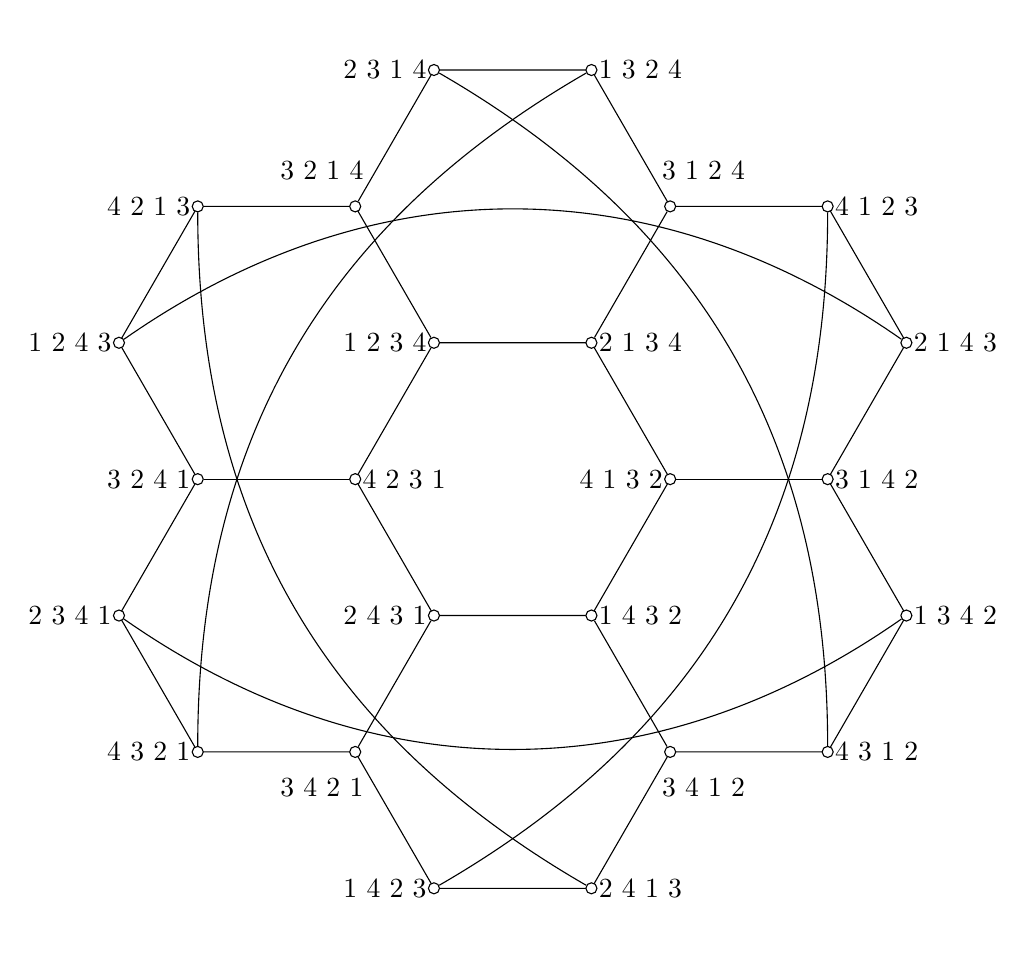
\begin{tikzpicture}
 		\tikzstyle{every node}=[draw,circle,fill=white,minimum size=4pt,inner sep=0pt]
 		\draw (0,0) node (1234) [label=left:$ 1\ 2\ 3\ 4$] {}
 		-- ++(0:2.0cm) node (2134) [label=right:$ 2\ 1\ 3\ 4$] {}
 		-- ++(300:2.0cm) node (4132) [label=left:$ 4\ 1\ 3\ 2$] {}
 		-- ++(240:2.0cm) node (1432) [label=right:$ 1\ 4\ 3\ 2$] {}
 		-- ++(180:2.0cm) node (2431) [label=left:$ 2\ 4\ 3\ 1$] {}
 		-- ++(120:2.0cm) node (4231) [label=right:$ 4\ 2\ 3\ 1$] {}
 		-- (1234) 
 		-- ++(120:2.0cm) node (3214) [label=120:$ 3\ 2\ 1\ 4$] {};
 		
 		\draw (3214)
 		-- ++(60:2.0cm) node (2314) [label=left:$ 2\ 3\ 1\ 4$] {}
 		-- ++(0:2.0cm) node (1324) [label=right:$ 1\ 3\ 2\ 4$] {}
 		-- ++(300:2.0cm) node (3124) [label=60:$ 3\ 1\ 2\ 4$] {}
 		-- ++(0:2.0cm) node (4123) [label=right:$ 4\ 1\ 2\ 3$] {}
 		-- ++(300:2.0cm) node (2143) [label=right:$ 2\ 1\ 4\ 3$] {}
 		-- ++(240:2.0cm) node (3142) [label=right:$ 3\ 1\ 4\ 2$] {}
 		-- ++(300:2.0cm) node (1342) [label=right:$ 1\ 3\ 4\ 2$] {}
 		-- ++(240:2.0cm) node (4312) [label=right:$ 4\ 3\ 1\ 2$] {}
 		-- ++(180:2.0cm) node (3412) [label=-60:$ 3\ 4\ 1\ 2$] {}
 		-- ++(240:2.0cm) node (2413) [label=right:$ 2\ 4\ 1\ 3$] {}
 		-- ++(180:2.0cm) node (1423) [label=left:$ 1\ 4\ 2\ 3$] {}
 		-- ++(120:2.0cm) node (3421) [label=-120:$ 3\ 4\ 2\ 1$] {}
 		-- ++(180:2.0cm) node (4321) [label=left:$ 4\ 3\ 2\ 1$] {}
 		-- ++(120:2.0cm) node (2341) [label=left:$ 2\ 3\ 4\ 1$] {}
 		-- ++(60:2.0cm) node (3241) [label=left:$ 3\ 2\ 4\ 1$] {}
 		-- ++(120:2.0cm) node (1243) [label=left:$ 1\ 2\ 4\ 3$] {}
 		-- ++(60:2.0cm) node (4213) [label=left:$ 4\ 2\ 1\ 3$] {}
 		-- (3214);
 		

 		\draw (3241) -- (4231);
 		\draw (3421) -- (2431);
 		\draw (1432) -- (3412);
 		\draw (4132) -- (3142);
 		\draw (2134) -- (3124);
 		

 		\draw (2341) to [out=-35,in=215] (1342);
 		\draw (1243) to [out=35,in=-215] (2143);
 		\draw (4123) to [out=270,in=30] (1423);
 		\draw (2314) to [out=-30,in=90] (4312);
 		\draw (1324) to [out=210,in=90] (4321);
 		\draw (4213) to [out=270,in=150] (2413);
 	\end{tikzpicture}
 \end{center}
\\
\par
\textbf{Grafic Desargues}
\par
Numele „grafic Desargues” a fost folosit și pentru a se referi la un grafic cu zece vârfuri, complementul graficului Petersen, care poate fi format și ca jumătate bipartită a graficului Desargues cu 20 de vârfuri.
\par
 \begin{center}
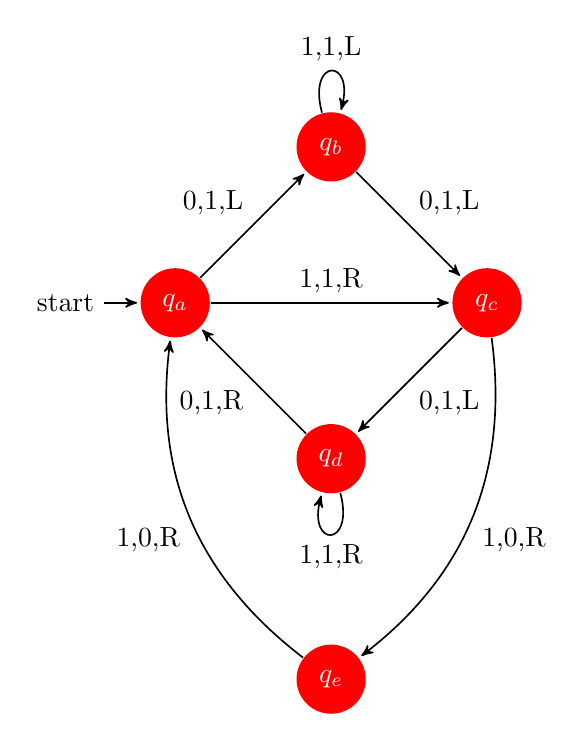
\begin{tikzpicture}[->,>=stealth',shorten >=1pt,auto,node distance=2.8cm,
	semithick]
	\tikzstyle{every state}=[fill=red,draw=none,text=white]
	
	\node[initial,state] (A)                    {$q_a$};
	\node[state]         (B) [above right of=A] {$q_b$};
	\node[state]         (D) [below right of=A] {$q_d$};
	\node[state]         (C) [below right of=B] {$q_c$};
	\node[state]         (E) [below of=D]       {$q_e$};
	
	\path (A) edge              node {0,1,L} (B)
	edge              node {1,1,R} (C)
	(B) edge [loop above] node {1,1,L} (B)
	edge              node {0,1,L} (C)
	(C) edge              node {0,1,L} (D)
	edge [bend left]  node {1,0,R} (E)
	(D) edge [loop below] node {1,1,R} (D)
	edge              node {0,1,R} (A)
	(E) edge [bend left]  node {1,0,R} (A);
\end{tikzpicture}
 \end{center}
\end{document}